% hello.tax - Our first LaTex example!

\documentclass[11pt]{article}
\setlength{\topmargin}{-0.25in}
\setlength{\headheight}{0in}
\setlength{\textheight}{9.5in}
\setlength{\headsep}{0in}
\setlength{\oddsidemargin}{-0.25in}
\setlength{\evensidemargin}{-0.25in}
\setlength{\textwidth}{7.0in}
\usepackage{times}
\usepackage{graphicx}
\usepackage{graphics}
\usepackage{epsfig}
\usepackage{url}
\usepackage{subfigure}
\usepackage{natbib}
\usepackage{amsmath,varwidth,array,ragged2e}

\newcolumntype{L}{>{\varwidth[c]{\linewidth}}l<{\endvarwidth}}
\newcolumntype{M}{>{$}l<{$}}
\def\ds{\mathrm{d}s}%  don't know what your \ds should be ....

\large\begin{document}

\title{MILEPOST GCC: machine learning based research compiler}
\author{Nilang Shah\\
  IIT Bombay, \\
  \em{Mumbai}, \\
  \textbf{shahnilang@cse.iitb.ac.in}}

\date{\today}
\maketitle

\begin{abstract}
Tuning hardwired compiler optimizations for rapidly
evolving hardware makes porting an optimizing com-
piler for each new platform extremely challenging. Our
radical approach is to develop a modular, extensible,
self-optimizing compiler that automatically learns the
best optimization\cite{LCTES} heuristics based on the behavior of the
platform. In this paper we describe MILEPOST1 GCC,
a machine-learning-based compiler that automatically
adjusts its optimization heuristics to improve the exe-
cution time, code size, or compilation time of specific
programs on different architectures. Our preliminary
experimental results show that it is possible to consider-
ably reduce execution time of the MiBench benchmark
suite on a range of platforms entirely automatically.
  \end{abstract}
\clearpage
\tableofcontents
\clearpage

\section{Introduction}

Current architectures and compilers continue to evolve
bringing higher performance, lower power and smaller
size while attempting to keep time to market as short as
possible.\cite{Plug} Typical systems may now have multiple het-
erogeneous reconfigurable cores and a great number of
compiler optimizations available, making manual com-
piler tuning increasingly infeasible. Furthermore, static
compilers often fail to produce high-quality code due to
a simplistic model of the underlying hardware.\\

A key goal of the project is to make machine learning
based compilation a realistic technology for general-
purpose compilation. Current approaches 
are highly preliminary limited to global compiler
flags or simple transformations considered in isolation.
GCC was selected as the compiler infrastructure for
MILEPOST as it is currently the most stable and ro-
bust open-source compiler.\cite{Qlogic} It supports multiple archi-
tectures and has multiple aggressive optimizations mak-
ing it a natural vehicle for our research. In addition,
each new version usually features new transformations
demonstrating the need for a system to automatically re-
tune its optimization heuristics.




\section{Structure}
Current architectures and compilers continue to evolve
bringing higher performance, lower power and smaller
size while attempting\cite{Mibench} to keep time to market as short as
possible. Typical systems may now have multiple het-
erogeneous reconfigurable cores and a great number of
compiler optimizations available, making manual com-
piler tuning increasingly infeasible. Furthermore, static
compilers often fail to produce high-quality code due to
a simplistic model of the underlying hardware.\\

In this paper we present early experimental results
showing that it is possible to improve the performance
of the well-known MiBench \cite{Auth09} benchmark suite on a
range of platforms including x86 and IA64. We ported
our tools to the new ARC GCC 4.2.1 that targets ARC
International’s configurable core family. Using MILE-
POST GCC, after a few weeks training, we were able to
learn a model that automatically improves the execution
time of MiBench benchmark by 11\% demonstrating the
use of our machine learning based compiler.\\

This paper is organized as follows: the next section de-
scribes the overall MILEPOST framework and is, it-
self, followed by a section detailing our implementation
of the Interactive Compilation Interface for GCC that
enables dynamic manipulation of optimization passes.
Section 4 describes machine learning techniques used
to predict \cite{ESTO} good optimization passes for programs us-
ing static program features and optimization knowledge
reuse. Section 5 provides experimental results and is
followed by concluding remarks.

\section{MILEPOST Framework}
The MILEPOST project uses a number of components,
at the heart of which is the machine learning enabled
MILEPOST GCC, shown in Fig.~\ref{fig-framestruct}. MILEPOST
GCC currently proceeds in two distinct phases, in ac-
cordance with typical machine learning practice: train-
ing and deployment.\\

\bf{Training}  \rm During the training phase we need to gather
information about the structure of programs and record
how they behave when compiled under different op-
timization settings.\cite{CCCF} Such information allows machine
learning tools to correlate aspects of program structure,
or \emph{features}, with optimizations, building a strategy that
predicts a good combination of optimizations.\\

In order to learn a good strategy, machine learning tools
need a large number of compilations and executions as
training examples. These training examples are gener-
ated by a tool, the Continuous Collective Compilation
Framework \cite{Midatasets}(CCC), which evaluates different compi-
lation optimizations, storing execution time, code size
and other metrics in a database. The features of the pro-
gram are extracted from MILEPOST GCC via a plugin
and are also stored in the database. Plugins allow fine
grained control and examination of the compiler, driven
externally through shared libraries.\\

\bf{Deployment} \rm Once sufficient training data is gathered,
a model is created using machine learning modeling.
The model is able to predict good optimization strate-
gies for a given set of program features and is built as
a plugin so that it can be re-inserted into MILEPOST
GCC. On encountering a new program the plugin deter-
mines the program’s features, passing them to the model
which determines the optimizations to be applied.\\

\bf{Framework} \rm In this paper we use a new version of the
Interactive Compilation Interface (ICI) for GCC which
controls the internal optimization decisions and their pa-
rameters using external plugins. It now allows the com-
plete substitution of default internal optimization heuris-
tics as well as the order of transformations.\\

\pagebreak
 
We use the Continuous Collective Compilation Frame-
work \cite{Mono08} to produce a training set for machine learn-
ing models to learn how to optimize programs for the
best performance, code size, power consumption and
any other objective function needed by the end-user.
This framework allows knowledge of the optimization
space to be reused among different programs, architec-
tures and data sets.\\

Together with additional routines needed for machine
learning, such as program feature extraction, this forms
the MILEPOST GCC. MILEPOST GCC transforms
the compiler suite into a powerful research tool suitable
for adaptive computing.\\

The next section describes the new ICI structure and ex-
plains how program features can be extracted for later
machine learning in Section 4.

\begin{figure}[ht]
\centering
  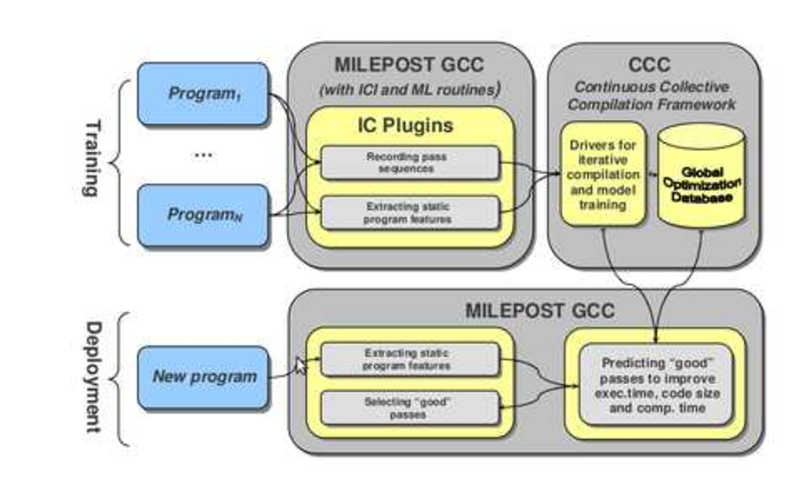
\includegraphics[scale =1]{Images/fig1}
\caption{Framework to automatically tune programs and improve default optimization heuristics using machine
learning techniques, MILEPOST GCC with Interactive Compilation Interface (ICI) and program features extractor,
and Continuous Collective Compilation Framework to train ML model and predict good optimization passes}
  \label{fig-framestruct}
 \end{figure}

\section{Interactive Compilation Interface}
%Set up an 'itemize' environment to start a bulleted list.  Each
%individual item begins with the \item command.  Also note in this list
%that it has two levels, with a list embedded in one of the list items.
This section describes the Interactive Compilation Inter-
face (ICI). The ICI provides opportunities for external
control and examination of the compiler. Optimization
settings at a fine-grained level, beyond the capabilities
of command line options or pragmas, can be managed
through external shared libraries, leaving the compiler
uncluttered.\\

The first version of ICI [21] was reactive and required
minimal changes to GCC. It was, however, unable to
modify the order of optimization passes within the com-
piler and so large opportunities for speedup were closed
to it. The new version of ICI [9] expands on the ca-
pabilities of its predecessor permitting the pass order to
be modified. This version of ICI is used in the MILE-
POST GCC to automatically learn good sequences of
optimization passes. In replacing default optimization
heuristics, execution time, code size and compilation
time can be improved.\\

\clearpage

\begin{enumerate}
\item {\bf AMD-} a cluster with 16 AMD Athlon 64 3700+
processors running at 2.4GHz
\item {\bf IA32-} a cluster with 4 Intel Xeon processors run-
ning at 2.8GHz
\item {\bf IA64 -} a server with Itanium2 processor running at
1.3GHz.
\item {\bf ARC -} FPGA implementation of the ARC 725D
processor running GNU/Linux with a 2.4.29 ker-
nel.
\end{enumerate}

\subsection{Internal structure}
To avoid the drawbacks of the first version of the ICI, we
designed a new version, as shown in Figure 2. This ver-
sion can now transparently monitor execution of passes
or replace the GCC Controller (Pass Manager), if de-
sired. Passes can be selected by an external plugin
which may choose to drive them in a very different order
to that currently used in GCC, even choosing different
pass orderings for each and every function in program
being compiled. Furthermore, the plugin can provide its
own passes, implemented entirely outside of GCC.\\

In an additional set of enhancements, a coherent event
and data passing mechanism enables external plugins to
discover the state of the compiler and to be informed as
it changes. At various points in the compilation process
events (IC Event) are raised indicating decisions about
transformations. Auxiliary data (IC Data) is registered
if needed.\\

Since plugins now extend GCC through external shared
libraries, experiments can be built with no further mod-
ifications to the underlying compiler. Modifications for\\

\begin{figure}[ht]
\centering
  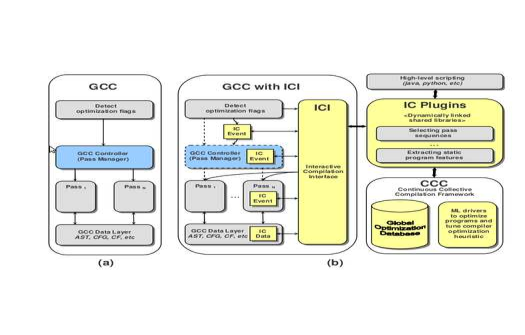
\includegraphics[scale =1]{Images/fig2}
\caption{GCC Interactive Compilation Interface: a) original GCC, b) GCC with ICI and plugins}
  \label{fig-framestruct2}
 \end{figure}

different analysis, optimization and monitoring scenar-
ios proceed in a tight engineering environment. These
plugins communicate with external drivers and can al-
low both high-level scripting and communication with
machine learning frameworks such as MILEPOST
GCC.\\

Note that it is not the goal of this project to develop
fully fledged plugin system. Rather, we show the util-
ity of such approaches for iterative compilation and
machine learning in compilers. We may later utilize
GCC plugin systems currently in development, for ex-
ample \cite{my}.\\

\subsection{Dynamic Manipulation of GCC Passes}
Previous research shows a great potential to improve
program execution time or reduce code size by carefully
selecting global compiler flags or transformation param-
eters using iterative compilation. The quality of gener-
ated code can also be improved by selecting different
optimization orders. Our
approach combine the selection of optimal optimization
orders and tuning parameters of transformations at the
same time.\\

Before we attempt to learn good optimization settings
and pass orders we first confirmed that there is indeed
performance to be gained within GCC from such actions
otherwise there is no point in trying to learn. By using
the Continuous Collective Compilation Framework
to random search though the optimization flag space
(50\% probability of selecting each optimization flag)
and MILEPOST GCC 4.2.2 on AMD Athlon64 3700+
and Intel Xeon 2800MHz we could improve execution
time of susan\_corners by around 16\%, compile time by
22\% and code size by 13\% using Pareto optimal points
as described in the previous work. Note, that
the same combination of flags degrade execution time
of this benchmark on Itanium-2 1.3GHz by 80 \% thus
demonstrating the importance of adapting compilers to
each new architecture. Figure 4a shows the combina-
tion of flags found for this benchmark on AMD platform
while Figures 4b,c show the passes invoked and moni-
tored by MILEPOST GCC for the default -O3 level and
for the best combination of flags respectively.\\

To verify that we can change the default optimization
pass orders using ICI, we recompiled the same bench-
mark with the -O3 flag but selecting passes.
 However, note that the GCC internal function
\emph{execute\_one\_pass} \rm has gate control
\emph{(pass $\rightarrow$ gate()) to execute the pass} \rm only if the associate
optimization flags is selected. To avoid this gate con-
trol we use \emph{IC-Parameter "gate\_status"}\rm and \emph{IC-Event
"avoid\_gate"}\rm so that we can set gate\_status to TRUE\\

within plugins and thus force its execution. The exe-
cution of the generated binary shows that we improve
its execution time by 13\% instead of 16\% and the rea-
son is that some compiler flags not only invoke associ-
ated pass such as -funroll-loops but also select specific
fine-grain transformation parameters and influence code
generation in other passes. Thus, at this point we recom-
pile programs with such flags always enabled, and in the
future plan to add support for such cases explicitly.

\section{Using Machine Learning to Select Good Optimization Passes}
The previous sections have described the infrastructure
necessary to build a learning compiler. In this section
we describe how this infrastructure is used in building a
model.\\

Our approach to selecting good passes for programs is
based upon the construction of a \emph{probabilistic model} on
a set of M training programs and the use of this model in
order to make predictions of “good” optimization passes
on unseen programs.\\

Our specific machine learning method is similar to that
of where a probability distribution over “good” so-
lutions (i.e. optimization passes or compiler flags) is
learnt across different programs. This approach has
been referred in the literature to as Predictive Search
Distributions (PSD). However, unlike 
where such a distribution is used to focus the search of
compiler optimizations on a new program, we use the
distribution learned to make one-shot predictions on un-
seen programs. Thus we do not search for the best opti-
mization, we automatically predict it.
\begin{figure}[ht]
\centering
  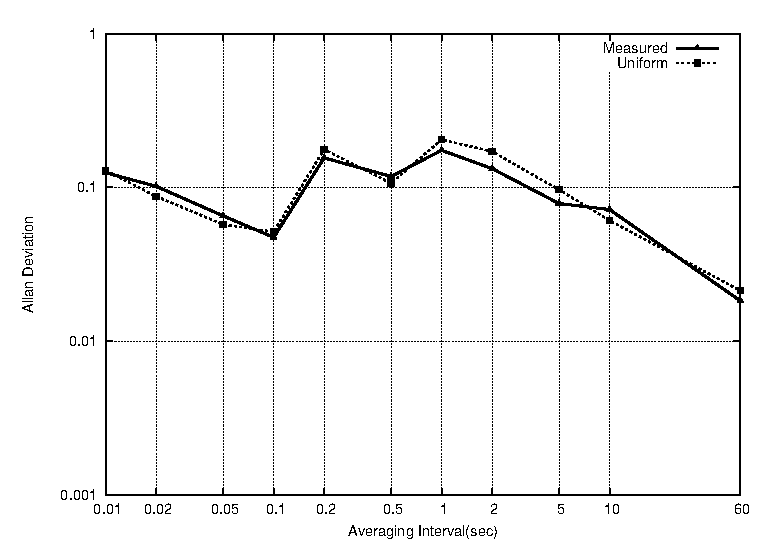
\includegraphics[scale =1]{plots/allan-dev}
\caption{plot1}
 \end{figure}
\subsection{The Machine Learning Model}
Given a set of training programs $T^1$ , . . . , $T^M$ , which can
be described by (vectors of) features $t^1$ . . . , $t^M$, and for
which we have evaluated different sequences of opti-
mization passes (x) and their corresponding execution
times (or speed-ups y) so that we have for each pro-
j
gram M j an associated dataset $D_j$ = ${({x}_{i}, {y}_{i})}_{i=1}^{N}$, with
j = 1, . . . M, our goal is to predict a good sequence of
optimization passes ${x}^{*}$ when a new program ${T}^{*}$ is pre-
sented.\\

We approach this problem by learning the mapping from
the features of a program t to a distribution over good
solutions $q(x|t, \theta)$, where θ are the parameters of the
distribution. Once this distribution has been learnt, pre-
dictions on a new program T ∗ is straightforward and it is
achieved by sampling at the mode of the distribution. In
other words, we obtain the predicted sequence of passes
by computing:\\

${P(x|{T}^{j} ) = \prod^{L}_{l=1} P(x |{T}^{j} ),}$\\
\def\arraystretch{1.7}
\begin{tabular}{rMrL}
(A) & \ds u=\sqrt{x^2+y^2} &(B) & $\ds u=\sqrt{x^4+y^4}$\tabularnewline
(C) & \ds u=\sqrt[3]{xy}   &(D) & $\ds u=\sqrt[3]{x^2+y^2}$\tabularnewline
(E) & \ds u=\sqrt[3]{x^4+y^4} & (F) & 
  \[ u=\begin{cases}e^{\frac{-1}{x^2+y^2}}; &x^2+y^2\neq 0\\ 0; &x^2+y^2=0\end{cases} \] \tabularnewline
(G) & \ds u=\sqrt[3]{x}\sin y & (H) & $\ds u=\sqrt[3]{y}\tan x$
\end{tabular}


\begin{figure}[ht]
\centering
  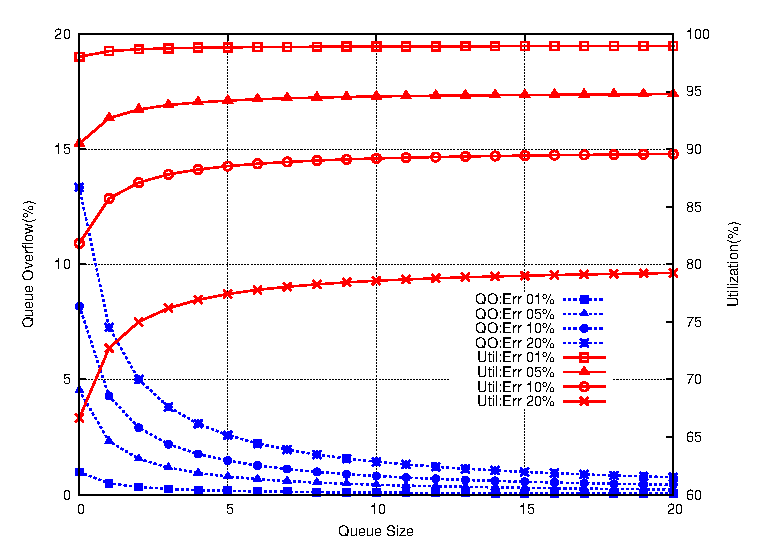
\includegraphics[scale =1]{plots/qsize-util-err}
\caption{plot2}
 \end{figure}



\bibliographystyle{plain}
\bibliography{paper}

\end{document}  %End of document.
